% Options for packages loaded elsewhere
% Options for packages loaded elsewhere
\PassOptionsToPackage{unicode}{hyperref}
\PassOptionsToPackage{hyphens}{url}
\PassOptionsToPackage{dvipsnames,svgnames,x11names}{xcolor}
%
\documentclass[
  letterpaper,
  DIV=11,
  numbers=noendperiod]{scrartcl}
\usepackage{xcolor}
\usepackage{amsmath,amssymb}
\setcounter{secnumdepth}{5}
\usepackage{iftex}
\ifPDFTeX
  \usepackage[T1]{fontenc}
  \usepackage[utf8]{inputenc}
  \usepackage{textcomp} % provide euro and other symbols
\else % if luatex or xetex
  \usepackage{unicode-math} % this also loads fontspec
  \defaultfontfeatures{Scale=MatchLowercase}
  \defaultfontfeatures[\rmfamily]{Ligatures=TeX,Scale=1}
\fi
\usepackage{lmodern}
\ifPDFTeX\else
  % xetex/luatex font selection
\fi
% Use upquote if available, for straight quotes in verbatim environments
\IfFileExists{upquote.sty}{\usepackage{upquote}}{}
\IfFileExists{microtype.sty}{% use microtype if available
  \usepackage[]{microtype}
  \UseMicrotypeSet[protrusion]{basicmath} % disable protrusion for tt fonts
}{}
\makeatletter
\@ifundefined{KOMAClassName}{% if non-KOMA class
  \IfFileExists{parskip.sty}{%
    \usepackage{parskip}
  }{% else
    \setlength{\parindent}{0pt}
    \setlength{\parskip}{6pt plus 2pt minus 1pt}}
}{% if KOMA class
  \KOMAoptions{parskip=half}}
\makeatother
% Make \paragraph and \subparagraph free-standing
\makeatletter
\ifx\paragraph\undefined\else
  \let\oldparagraph\paragraph
  \renewcommand{\paragraph}{
    \@ifstar
      \xxxParagraphStar
      \xxxParagraphNoStar
  }
  \newcommand{\xxxParagraphStar}[1]{\oldparagraph*{#1}\mbox{}}
  \newcommand{\xxxParagraphNoStar}[1]{\oldparagraph{#1}\mbox{}}
\fi
\ifx\subparagraph\undefined\else
  \let\oldsubparagraph\subparagraph
  \renewcommand{\subparagraph}{
    \@ifstar
      \xxxSubParagraphStar
      \xxxSubParagraphNoStar
  }
  \newcommand{\xxxSubParagraphStar}[1]{\oldsubparagraph*{#1}\mbox{}}
  \newcommand{\xxxSubParagraphNoStar}[1]{\oldsubparagraph{#1}\mbox{}}
\fi
\makeatother


\usepackage{longtable,booktabs,array}
\newcounter{none} % for unnumbered tables
\usepackage{calc} % for calculating minipage widths
% Correct order of tables after \paragraph or \subparagraph
\usepackage{etoolbox}
\makeatletter
\patchcmd\longtable{\par}{\if@noskipsec\mbox{}\fi\par}{}{}
\makeatother
% Allow footnotes in longtable head/foot
\IfFileExists{footnotehyper.sty}{\usepackage{footnotehyper}}{\usepackage{footnote}}
\makesavenoteenv{longtable}
\usepackage{graphicx}
\makeatletter
\newsavebox\pandoc@box
\newcommand*\pandocbounded[1]{% scales image to fit in text height/width
  \sbox\pandoc@box{#1}%
  \Gscale@div\@tempa{\textheight}{\dimexpr\ht\pandoc@box+\dp\pandoc@box\relax}%
  \Gscale@div\@tempb{\linewidth}{\wd\pandoc@box}%
  \ifdim\@tempb\p@<\@tempa\p@\let\@tempa\@tempb\fi% select the smaller of both
  \ifdim\@tempa\p@<\p@\scalebox{\@tempa}{\usebox\pandoc@box}%
  \else\usebox{\pandoc@box}%
  \fi%
}
% Set default figure placement to htbp
\def\fps@figure{htbp}
\makeatother


% definitions for citeproc citations
\NewDocumentCommand\citeproctext{}{}
\NewDocumentCommand\citeproc{mm}{%
  \begingroup\def\citeproctext{#2}\cite{#1}\endgroup}
\makeatletter
 % allow citations to break across lines
 \let\@cite@ofmt\@firstofone
 % avoid brackets around text for \cite:
 \def\@biblabel#1{}
 \def\@cite#1#2{{#1\if@tempswa , #2\fi}}
\makeatother
\newlength{\cslhangindent}
\setlength{\cslhangindent}{1.5em}
\newlength{\csllabelwidth}
\setlength{\csllabelwidth}{3em}
\newenvironment{CSLReferences}[2] % #1 hanging-indent, #2 entry-spacing
 {\begin{list}{}{%
  \setlength{\itemindent}{0pt}
  \setlength{\leftmargin}{0pt}
  \setlength{\parsep}{0pt}
  % turn on hanging indent if param 1 is 1
  \ifodd #1
   \setlength{\leftmargin}{\cslhangindent}
   \setlength{\itemindent}{-1\cslhangindent}
  \fi
  % set entry spacing
  \setlength{\itemsep}{#2\baselineskip}}}
 {\end{list}}
\usepackage{calc}
\newcommand{\CSLBlock}[1]{\hfill\break\parbox[t]{\linewidth}{\strut\ignorespaces#1\strut}}
\newcommand{\CSLLeftMargin}[1]{\parbox[t]{\csllabelwidth}{\strut#1\strut}}
\newcommand{\CSLRightInline}[1]{\parbox[t]{\linewidth - \csllabelwidth}{\strut#1\strut}}
\newcommand{\CSLIndent}[1]{\hspace{\cslhangindent}#1}



\setlength{\emergencystretch}{3em} % prevent overfull lines

\providecommand{\tightlist}{%
  \setlength{\itemsep}{0pt}\setlength{\parskip}{0pt}}



 


\KOMAoption{captions}{tableheading}
\makeatletter
\@ifpackageloaded{caption}{}{\usepackage{caption}}
\AtBeginDocument{%
\ifdefined\contentsname
  \renewcommand*\contentsname{Table of contents}
\else
  \newcommand\contentsname{Table of contents}
\fi
\ifdefined\listfigurename
  \renewcommand*\listfigurename{List of Figures}
\else
  \newcommand\listfigurename{List of Figures}
\fi
\ifdefined\listtablename
  \renewcommand*\listtablename{List of Tables}
\else
  \newcommand\listtablename{List of Tables}
\fi
\ifdefined\figurename
  \renewcommand*\figurename{Figure}
\else
  \newcommand\figurename{Figure}
\fi
\ifdefined\tablename
  \renewcommand*\tablename{Table}
\else
  \newcommand\tablename{Table}
\fi
}
\@ifpackageloaded{float}{}{\usepackage{float}}
\floatstyle{ruled}
\@ifundefined{c@chapter}{\newfloat{codelisting}{h}{lop}}{\newfloat{codelisting}{h}{lop}[chapter]}
\floatname{codelisting}{Listing}
\newcommand*\listoflistings{\listof{codelisting}{List of Listings}}
\makeatother
\makeatletter
\makeatother
\makeatletter
\@ifpackageloaded{caption}{}{\usepackage{caption}}
\@ifpackageloaded{subcaption}{}{\usepackage{subcaption}}
\makeatother
\usepackage{bookmark}
\IfFileExists{xurl.sty}{\usepackage{xurl}}{} % add URL line breaks if available
\urlstyle{same}
\hypersetup{
  pdftitle={A Decade of Decline: Confronting the Reality of Auckland's Dog Control Crisis Using Auckland Council Data},
  pdfauthor={Thomas E. Saunders},
  pdfkeywords={dog control, dog attacks, Auckland, euthanasia},
  colorlinks=true,
  linkcolor={blue},
  filecolor={Maroon},
  citecolor={Blue},
  urlcolor={Blue},
  pdfcreator={LaTeX via pandoc}}


\title{A Decade of Decline: Confronting the Reality of Auckland's Dog
Control Crisis Using Auckland Council Data}
\author{Thomas E. Saunders}
\date{2026-03-24}
\begin{document}
\maketitle
\begin{abstract}
A spate of fatal dog attacks have focussed attention on New Zealand's
growing problem with roaming and aggressive dogs. Under the Dog Control
Act 1996, Territorial Authorities are resposible for managing the harms
associated with dogs in communities. Auckland Council's Animal
Management division publishes selected high-level statistics related to
it's dog control practices, but an examination of the underlying raw
data in combination with data from it's annual reports reveals troubling
trends for some of the most important metrics. The rate of attacks,
impounds, and euthanasia of impounded dogs are all increasing due to an
explosion in the dog population and a stretched shelter system. Attack
rates are highest in South Auckland, and several breeds are
over-represented in negative statistics.
\end{abstract}


\section{Key Points}\label{key-points}

Over the last 10 years:

\begin{itemize}
\tightlist
\item
  Auckland's dog population has increased by 14.5\%, mostly since
  FY2020.
\item
  Registration and desexing rates have fallen, while the proportion of
  `menacing' dogs has doubled to 1 in 20.
\item
  Dog attack rates have almost doubled from 6 to 10 attacks for every
  1,000 dogs.
\item
  Impound rates in FY2025 are the second highest ever.
\item
  Euthanasia rates of impounded dogs have risen from 22\% to 60\%,
  mostly due to failed temperament tests and full shelters.
\item
  A small number of breeds are over-represented in attacks and impounds.
\item
  Local Boards in South Auckland have experienced lower rates of
  registration and desexing, and higher rates of attacks and impounds.
\end{itemize}

\section{Introduction}\label{introduction}

Four fatal dog attacks in New Zealand in the last four years have
highlighted the increase in roaming and aggressive dogs in communities
across the country.

\begin{itemize}
\tightlist
\item
  Neville Thomson was killed in Katikati in August 2022 after being
  mauled by a pack of dogs owned by Abel Wira, whose property Thomson
  was staying at\textsuperscript{1}.
\item
  Elizabeth Whittaker was killed in October 2023 in Moerewa, Northland,
  in her backyard by dogs owned by another resident at the
  property\textsuperscript{2}.
\item
  Timothy Tu'uaki Rolleston-Bryan, a four-year-old boy, died in March
  2025 following an attack on a Katikati property\textsuperscript{3}.
\item
  Mihiata Te Rore died following an attack by three dogs while visiting
  a property in Kaihu, Northland, in February 2026\textsuperscript{4}.
\end{itemize}

Recent media reports have drawn attention to dog attacks on other
animals: from packs of roaming dogs killing sheep and calves in
Northland\textsuperscript{5}, to the killing of dozens of pets in an
Auckland suburb\textsuperscript{6}. Blind Low Vision NZ is no longer
placing guide dogs in certain South Auckland areas due to the high rates
of dog attacks on guide dogs and their handlers\textsuperscript{7}.
Residents in South Auckland communities report living in
fear\textsuperscript{8}, with elderly residents afraid to leave their
homes, and children missing school for fear of encountering roaming
aggressive dogs on their way to school, or within school
grounds\textsuperscript{9}.

The Dog Control Act 1996\textsuperscript{10} defines the obligations of
dog owners, which include registering their dog, controlling their dog
at all times, and ensuring their dog ``does not injure, endanger,
intimidate, or otherwise cause distress to any person.'' The Act also
lays out the functions, duties, and powers of territorial authorities,
which include minimising the dangers presented by dogs in the community
and ensuring the public can ``use streets and public amenities without
fear of attack or intimidation by dogs.'' Auckland Council's approach to
dog control is set out in it's Dog Management Bylaw\textsuperscript{11}
and Policy on Dogs\textsuperscript{12}. Auckland Council's Animal
Management division has around 150 permanent staff, including five
area-based field teams (Central, East, North, South and West), a
regional Barking and Registration team, a Proactive team, four animal
shelters (Henderson, Manukau, Silverdale, and Pukekohe), a Veterinary
Services team, and management, legal, and operational support staff.

Territorial authorities are required to collect and publish data
relating to dog control policies and practices. Auckland Council's
Animal Management division publishes a high-level summary of selected
data in it's annual reports. I made a request under the Local Government
Official Information and Meetings Act 1987\textsuperscript{13} on 20
November 2025 for the full dataset compiled by the Council, which was
fulfilled on 18 December 2025 (request \#8140017948). The raw data is
available as an R package called \texttt{akldogs}\textsuperscript{14},
and the data is also available as cleaned .csv files in the package's
\href{https://github.com/tesaunders/akldogs/tree/main/data-raw}{GitHub
repository}. I also compiled data from Auckland Council Animal
Management annual reports going back to FY2016, and this data can be
found \href{./data}{here}. Below is an exploration of both data sources
to understand Auckland's dog population and it's management.

\section{Auckland Dog Population}\label{auckland-dog-population}

There were 131,123 known dogs in the Auckland region as at FY2025. As
the dog population has increased, rates of registration and desexing
have fallen. The proportion of dogs classified as `menacing' under the
Dog Control Act 1996, either due to their breed or behaviour, has
doubled since 2016 to 1 in 20 dogs. A drop in the recorded dog
population in 2018 was due to the removal of duplicate entries in the
Auckland Council dog database, and in 2025 was due to the updating of
the database during a registration campaign.

\protect\phantomsection\label{ownership-trends}
{\def\LTcaptype{none} % do not increment counter
\begin{longtable}[]{@{}rlllll@{}}
\toprule\noalign{}
Year & Known Dogs & Pop. Change (\%) & Registered (\%) & Desexed (\%) &
Menacing (\%) \\
\midrule\noalign{}
\endhead
\bottomrule\noalign{}
\endlastfoot
2025 & 131,123 & -3.4\% & 88.4\% & 65.0\% & 5.1\% \\
2024 & 135,546 & 2.8\% & 83.6\% & 66.4\% & 4.7\% \\
2023 & 131,795 & 5.1\% & 88.2\% & 68.2\% & 4.1\% \\
2022 & 125,016 & 5.2\% & 91.0\% & 50.7\% & 4.3\% \\
2021 & 118,552 & 5.1\% & 94.8\% & 73.4\% & 4.1\% \\
2020 & 112,530 & 1.4\% & 94.4\% & NA & 4.2\% \\
2019 & 110,969 & 0.9\% & 96.1\% & NA & 4.0\% \\
2018 & 110,012 & -5.0\% & 93.6\% & NA & 3.9\% \\
2017 & 115,544 & 0.9\% & 83.7\% & NA & 3.6\% \\
2016 & 114,519 & 4.1\% & 93.2\% & NA & 2.4\% \\
2015 & 109,840 & 4.3\% & 91.2\% & NA & 2.7\% \\
2014 & 105,095 & NA & 95.9\% & NA & 0.7\% \\
\end{longtable}
}

\textsubscript{Source:
\href{https://tesaunders.github.io/dog-control/notebooks/data-analysis-preview.html\#cell-ownership-trends}{Data
Analysis}}

Over 200 breeds are represented in the Auckland dog population. Labrador
Retrievers remain the most popular at 11\% of the Auckland dog
population, with the top 10 also including the Staffordshire Bull
Terrier and American Pit Bull Terrier, both automatically classified as
`menacing' under the Dog Control Act 1996.

\protect\phantomsection\label{top-breeds}
{\def\LTcaptype{none} % do not increment counter
\begin{longtable}[]{@{}lll@{}}
\toprule\noalign{}
Breed & Count & Proportion \\
\midrule\noalign{}
\endhead
\bottomrule\noalign{}
\endlastfoot
Labrador Retriever & 14,959 & 11.4\% \\
Staffordshire Bull Terrier & 8,474 & 6.5\% \\
Border Collie & 6,170 & 4.7\% \\
Miniature Schnauzer & 4,900 & 3.7\% \\
Cavalier King Charles Spaniel & 4,784 & 3.6\% \\
Golden Retriever & 4,636 & 3.5\% \\
Shih Tzu & 4,216 & 3.2\% \\
German Shepherd & 4,196 & 3.2\% \\
American Pit Bull Terrier & 3,908 & 3.0\% \\
Jack Russell Terrier & 3,641 & 2.8\% \\
\end{longtable}
}

\textsubscript{Source:
\href{https://tesaunders.github.io/dog-control/notebooks/data-analysis-preview.html\#cell-top-breeds}{Data
Analysis}}

\section{Dog Attacks}\label{dog-attacks}

The rate of dog attacks have almost doubled since 2016, from 6 attacks
for every 1,000 dogs, to 10 attacks for every 1,000 dogs in 2025.

\pandocbounded{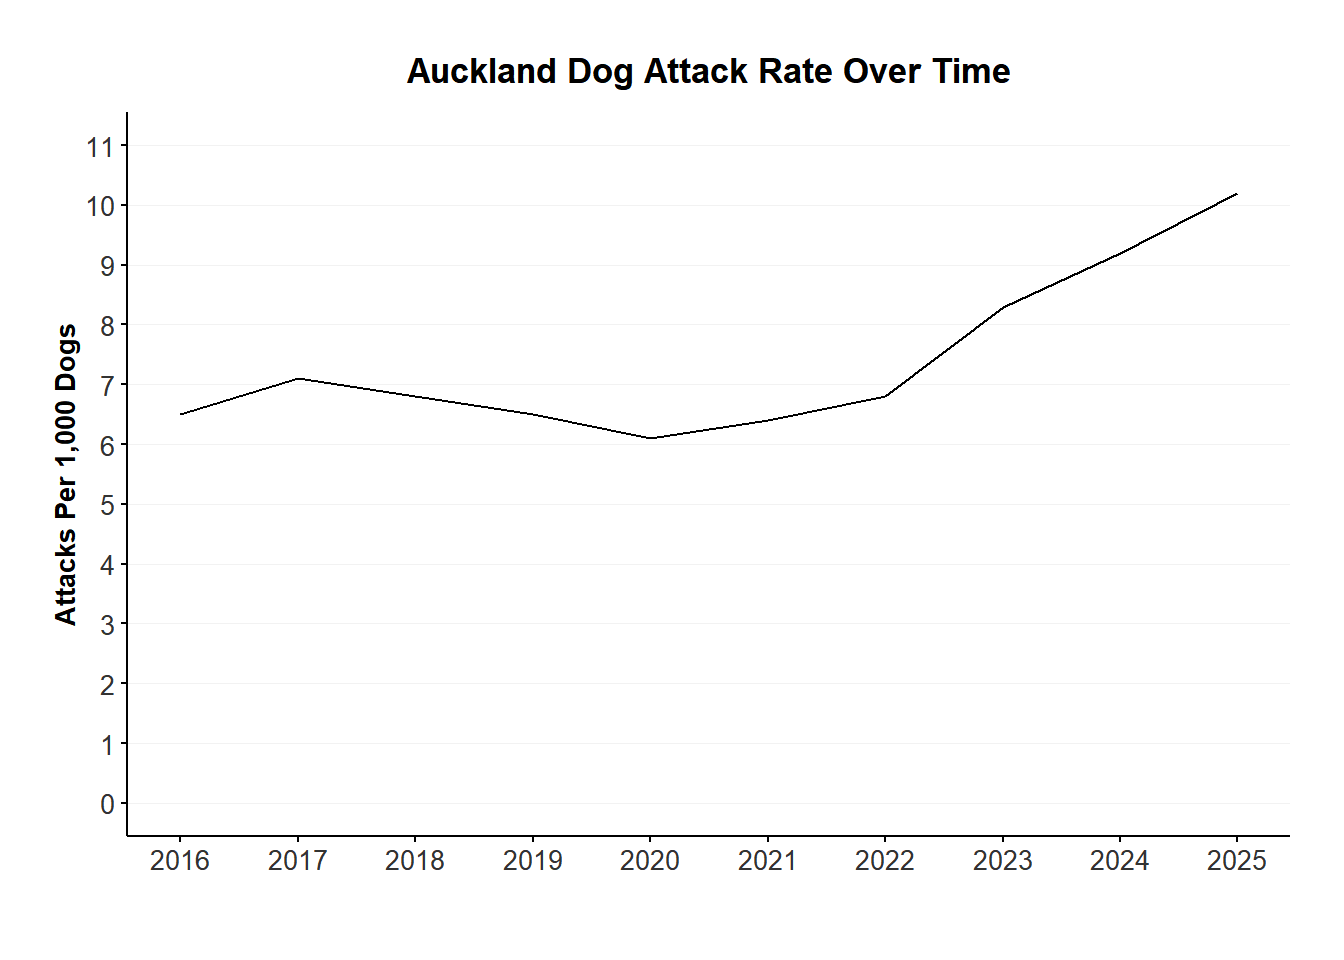
\includegraphics[keepaspectratio]{index_files/figure-latex/notebooks-data-analysis-attacks-plot-output-1.png}}

\textsubscript{Source:
\href{https://tesaunders.github.io/dog-control/notebooks/data-analysis-preview.html\#cell-attacks-plot}{Data
Analysis}}

When Auckland Council Animal Management officers impound a dog because
it has attacked a person, the attack severity is measured on a scale
from 0 to 5. In all impounds for attacks in 2024 (the most recent year
for the full impound data), Pit Bull Terriers or Staffordshire Terriers
were responsible for the highest or second highest numbers of attacks in
each severity category.

\section{Impounds}\label{impounds}

The rate of impounds per 1,000 dogs in the population reached 77.9 in
2025, the highest ever.

\protect\phantomsection\label{impound-rate}
{\def\LTcaptype{none} % do not increment counter
\begin{longtable}[]{@{}rllr@{}}
\toprule\noalign{}
Year & Known Dogs & Impounded Dogs & Impound Rate \\
\midrule\noalign{}
\endhead
\bottomrule\noalign{}
\endlastfoot
2025 & 131,123 & 10,214 & 77.9 \\
2024 & 135,546 & 8,306 & 61.3 \\
2023 & 131,795 & 6,596 & 50.0 \\
2022 & 125,016 & 5,012 & 40.1 \\
2021 & 118,552 & 5,228 & 44.1 \\
2020 & 112,530 & 5,492 & 48.8 \\
2019 & 110,969 & 6,833 & 61.6 \\
2018 & 110,012 & 7,457 & 67.8 \\
2017 & 115,544 & 8,416 & 72.8 \\
2016 & 114,519 & 8,614 & 75.2 \\
2015 & 109,840 & 9,432 & 85.9 \\
2014 & 105,095 & 7,373 & 70.2 \\
\end{longtable}
}

\textsubscript{Source:
\href{https://tesaunders.github.io/dog-control/notebooks/data-analysis-preview.html\#cell-impound-rate}{Data
Analysis}}

The rate of impounds differed markedly by breed, with a 3 times
difference even within the top 10.

\protect\phantomsection\label{impounds-breed}
{\def\LTcaptype{none} % do not increment counter
\begin{longtable}[]{@{}lllr@{}}
\toprule\noalign{}
Breed & Impounds & Population & Impound Rate \\
\midrule\noalign{}
\endhead
\bottomrule\noalign{}
\endlastfoot
Mastiff & 486 & 1,526 & 318.5 \\
Staffordshire Bull Terrier & 1,972 & 8,474 & 232.7 \\
Shar Pei & 494 & 2,445 & 202.0 \\
American Bulldog & 285 & 1,707 & 167.0 \\
American Staffordshire Terrier & 336 & 2,297 & 146.3 \\
Bearded Collie & 91 & 673 & 135.2 \\
Siberian Husky & 149 & 1,330 & 112.0 \\
Catahoula Leopard & 24 & 228 & 105.3 \\
Neapolitan Mastiff & 29 & 293 & 99.0 \\
Huntaway & 300 & 3,191 & 94.0 \\
\end{longtable}
}

\textsubscript{Source:
\href{https://tesaunders.github.io/dog-control/notebooks/data-analysis-preview.html\#cell-impounds-breed}{Data
Analysis}}

The proportion of impounded dogs that were euthanised was steadily
dropping between 2014 and 2021, when it reached a low of 21.7\%.
However, since then it climbed dramatically to reach 60.8\% in 2025.

\pandocbounded{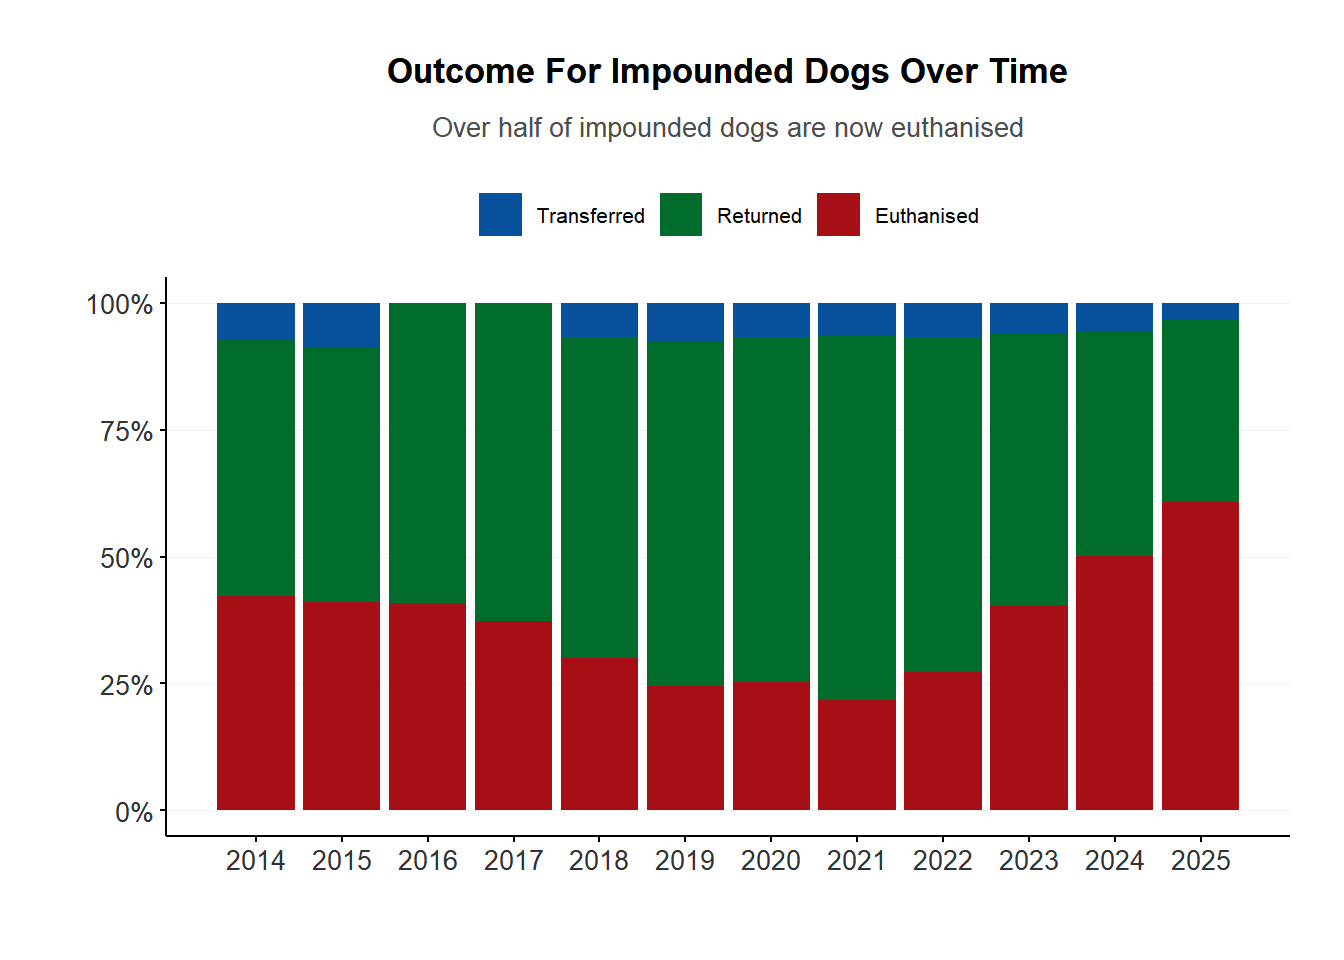
\includegraphics[keepaspectratio]{index_files/figure-latex/notebooks-data-analysis-impound-outcome-output-2.png}}

\textsubscript{Source:
\href{https://tesaunders.github.io/dog-control/notebooks/data-analysis-preview.html\#cell-impound-outcome}{Data
Analysis}}

Most seized or uncollected dogs were euthanised because they failed a
temperament test (50.1\%), and were therefore unsuitable for adoption.
But a quarter of euthanised dogs were put down because the animal
shelter was full.

Some dog breeds were significantly over-represented in euthanised dogs
compared to the overall dog population. For example, Staffordshire Bull
Terriers made up just over 6\% of the dog population in 2024, but
accounted for just over 30\% of euthanised dogs in animal shelters. On
the other hand, breeds like Labrador Retrievers were under-represented,
making up just over 11\% of the population but accounting for under 8\%
of euthanised dogs.

\pandocbounded{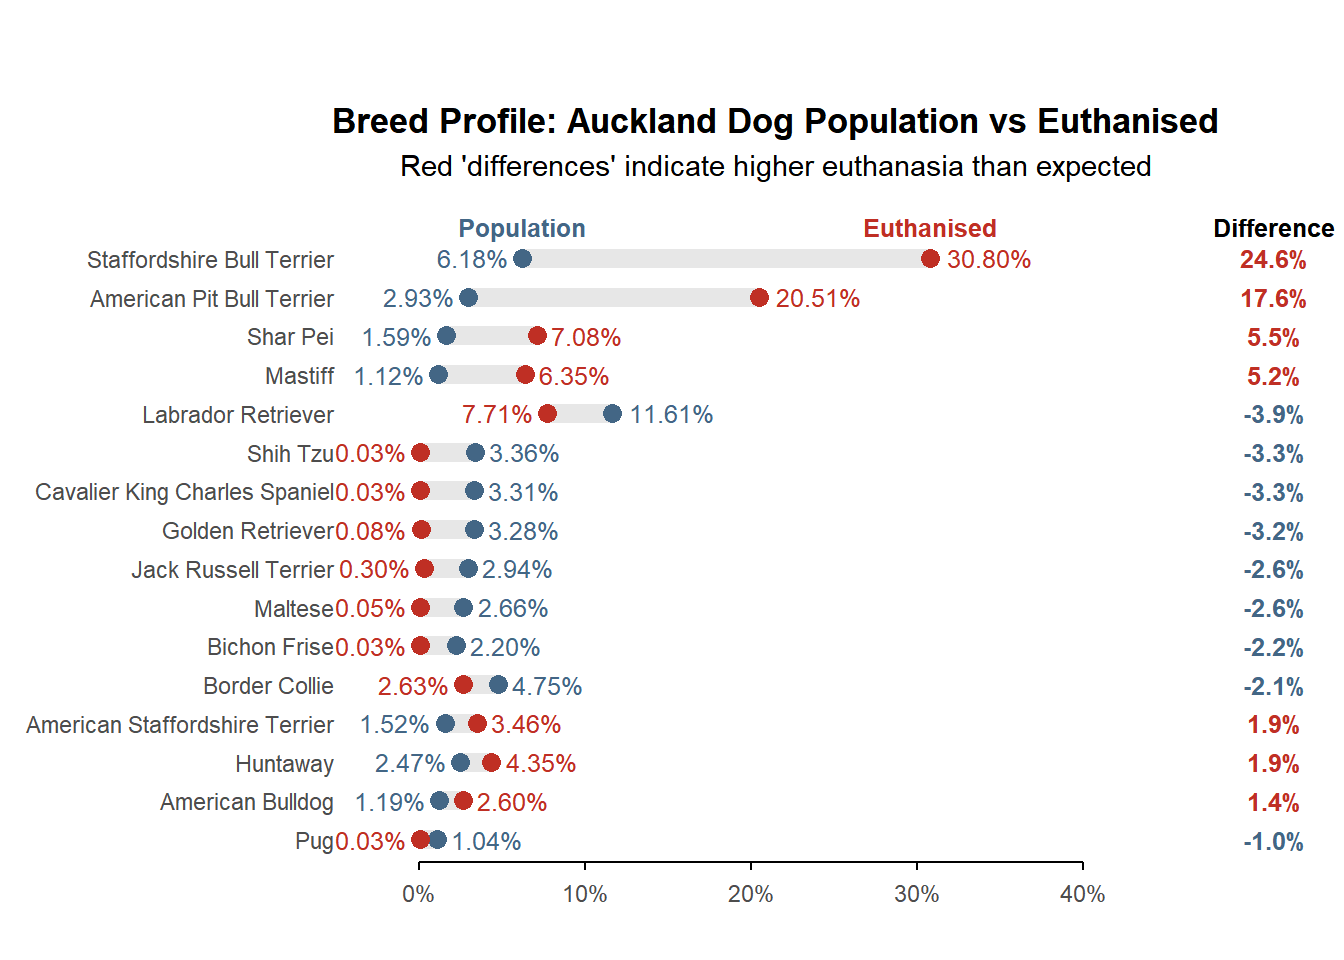
\includegraphics[keepaspectratio]{index_files/figure-latex/notebooks-data-analysis-euth-breed-output-1.png}}

\textsubscript{Source:
\href{https://tesaunders.github.io/dog-control/notebooks/data-analysis-preview.html\#cell-euth-breed}{Data
Analysis}}

\section{Compliance}\label{compliance}

The number of infringements issued by Animal Management officers under
the Dog Control Act 1996 tripled between 2024 and 2025, from 6,387 to
17,430, the majority of which were failure to register a dog. Despite
this, the number of prosecutions and appeals brought by Animal
Management has dropped from around 197 in 2016 to 141 in 2025.

\section{Regional Statistics}\label{regional-statistics}

Auckland's 21 Local Boards can be grouped into 5 regions (north, south,
east, west, central).

\protect\phantomsection\label{map-regions-boards}

\textsubscript{Source:
\href{https://tesaunders.github.io/dog-control/notebooks/mapping-preview.html\#cell-map-regions-boards}{Mapping}}

Regional dog population.

\protect\phantomsection\label{region-pop}
{\def\LTcaptype{none} % do not increment counter
\begin{longtable}[]{@{}ll@{}}
\toprule\noalign{}
Region & Dogs \\
\midrule\noalign{}
\endhead
\bottomrule\noalign{}
\endlastfoot
north & 43,051 \\
south & 33,754 \\
central & 25,368 \\
west & 20,046 \\
east & 8,904 \\
\end{longtable}
}

\textsubscript{Source:
\href{https://tesaunders.github.io/dog-control/notebooks/data-analysis-preview.html\#cell-region-pop}{Data
Analysis}}

Between 2021 and 2025, all Local Board areas experienced an increase in
their dog population. While the median increase was 9\%, Māngere-Ōtāhuhu
and Ōtara-Papatoetoe Local Boards had significantly higher growth based
on an analysis of the interquartile range.

\protect\phantomsection\label{board-pop}
{\def\LTcaptype{none} % do not increment counter
\begin{longtable}[]{@{}lllllll@{}}
\toprule\noalign{}
Local Board & 2021 & 2022 & 2023 & 2024 & 2025 & Change \\
\midrule\noalign{}
\endhead
\bottomrule\noalign{}
\endlastfoot
Māngere-Ōtāhuhu Local Board Area & 3,407 & 3,677 & 4,173 & 4,670 & 4,809
& 41.2\% \\
Ōtara-Papatoetoe Local Board Area & 3,912 & 4,267 & 4,668 & 5,107 &
5,192 & 32.7\% \\
Maungakiekie-Tāmaki Local Board Area & 4,540 & 4,882 & 5,226 & 5,514 &
5,484 & 20.8\% \\
Aotea/Great Barrier Local Board Area & 295 & 301 & 325 & 341 & 349 &
18.3\% \\
Manurewa Local Board Area & 5,043 & 5,306 & 5,589 & 5,923 & 5,808 &
15.2\% \\
Henderson-Massey Local Board Area & 9,140 & 9,514 & 10,067 & 10,440 &
10,288 & 12.6\% \\
Upper Harbour Local Board Area & 4,880 & 5,307 & 5,607 & 5,696 & 5,464 &
12.0\% \\
Puketāpapa Local Board Area & 1,954 & 2,080 & 2,227 & 2,282 & 2,180 &
11.6\% \\
Whau Local Board Area & 3,337 & 3,493 & 3,690 & 3,817 & 3,694 &
10.7\% \\
Hibiscus and Bays Local Board Area & 11,369 & 12,035 & 12,621 & 12,994 &
12,529 & 10.2\% \\
Kaipātiki Local Board Area & 5,753 & 6,088 & 6,458 & 6,534 & 6,275 &
9.1\% \\
Albert-Eden Local Board Area & 5,726 & 6,128 & 6,427 & 6,498 & 6,233 &
8.9\% \\
Howick Local Board Area & 8,228 & 8,672 & 9,145 & 9,275 & 8,904 &
8.2\% \\
Waitematā Local Board Area & 4,014 & 4,295 & 4,462 & 4,554 & 4,310 &
7.4\% \\
Papakura Local Board Area & 5,565 & 5,859 & 6,091 & 6,281 & 5,967 &
7.2\% \\
Devonport-Takapuna Local Board Area & 4,290 & 4,423 & 4,720 & 4,799 &
4,592 & 7.0\% \\
Franklin Local Board Area & 11,218 & 11,879 & 12,426 & 12,560 & 11,978 &
6.8\% \\
Waitākere Ranges Local Board Area & 5,729 & 5,961 & 6,211 & 6,302 &
6,064 & 5.8\% \\
Ōrākei Local Board Area & 6,810 & 7,096 & 7,403 & 7,516 & 7,161 &
5.2\% \\
Rodney Local Board Area & 12,152 & 12,555 & 12,976 & 13,245 & 12,635 &
4.0\% \\
Waiheke Local Board Area & 1,180 & 1,200 & 1,271 & 1,272 & 1,207 &
2.3\% \\
\end{longtable}
}

\textsubscript{Source:
\href{https://tesaunders.github.io/dog-control/notebooks/data-analysis-preview.html\#cell-board-pop}{Data
Analysis}}

Local Board areas differed greatly on rates of registration, desexing,
dogs classified as menacing or dangerous, and the proportion of owners
with a Responsible Dog Owner Licence.

A Spearman rank correlation analysis showed that Local Boards with high
current registrations tended to have higher rates of desexing and lower
rates of classified animals, while those with higher rates of
classifications tended to have lower rates of desexing.

\pandocbounded{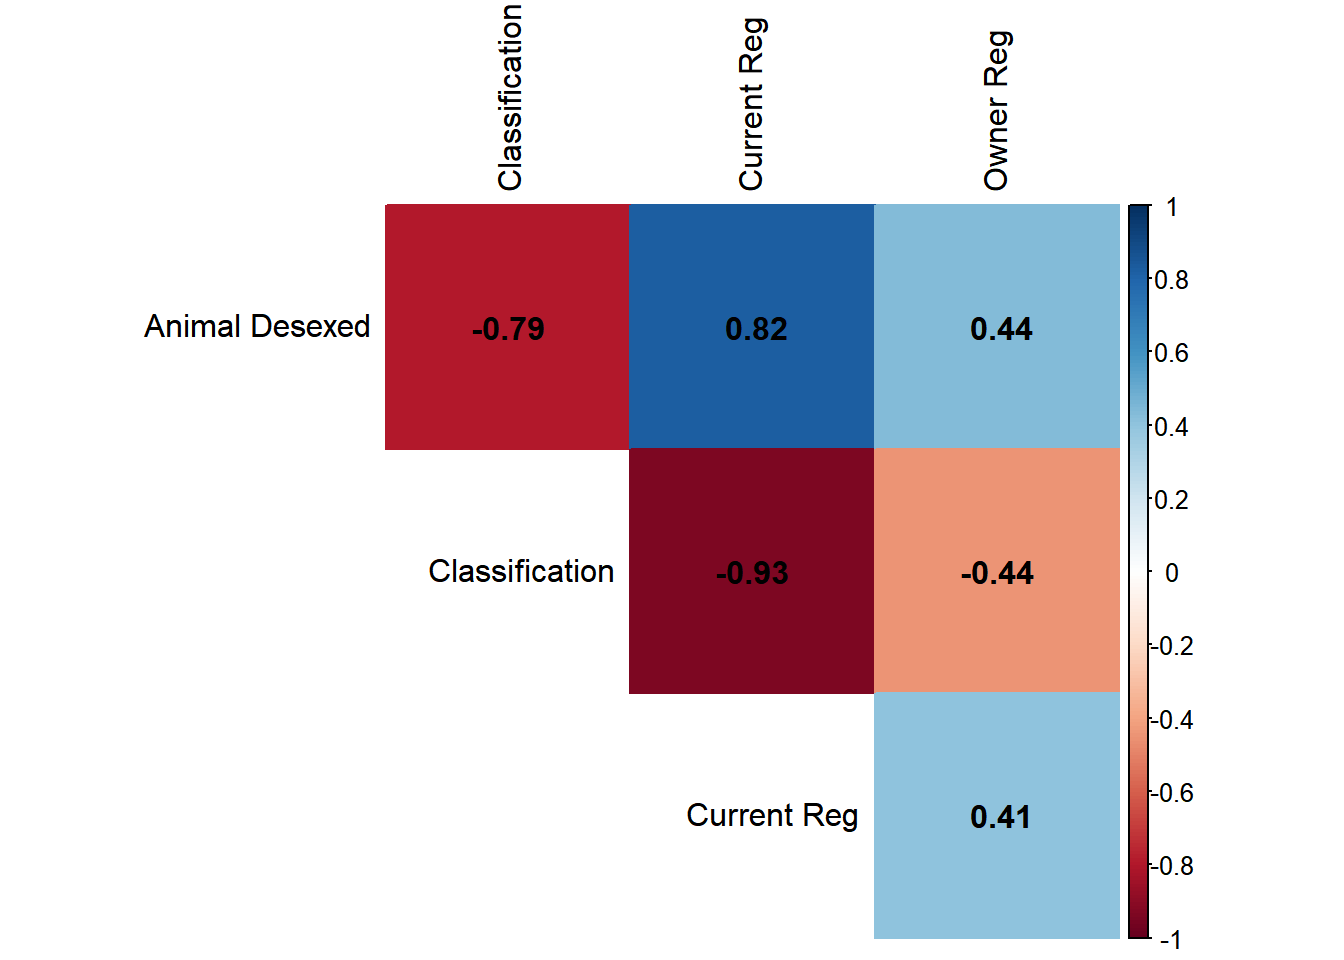
\includegraphics[keepaspectratio]{index_files/figure-latex/notebooks-data-analysis-spearman-output-1.png}}

\textsubscript{Source:
\href{https://tesaunders.github.io/dog-control/notebooks/data-analysis-preview.html\#cell-spearman}{Data
Analysis}}

Local Boards differed in rates of desexing and classified dogs.

\pandocbounded{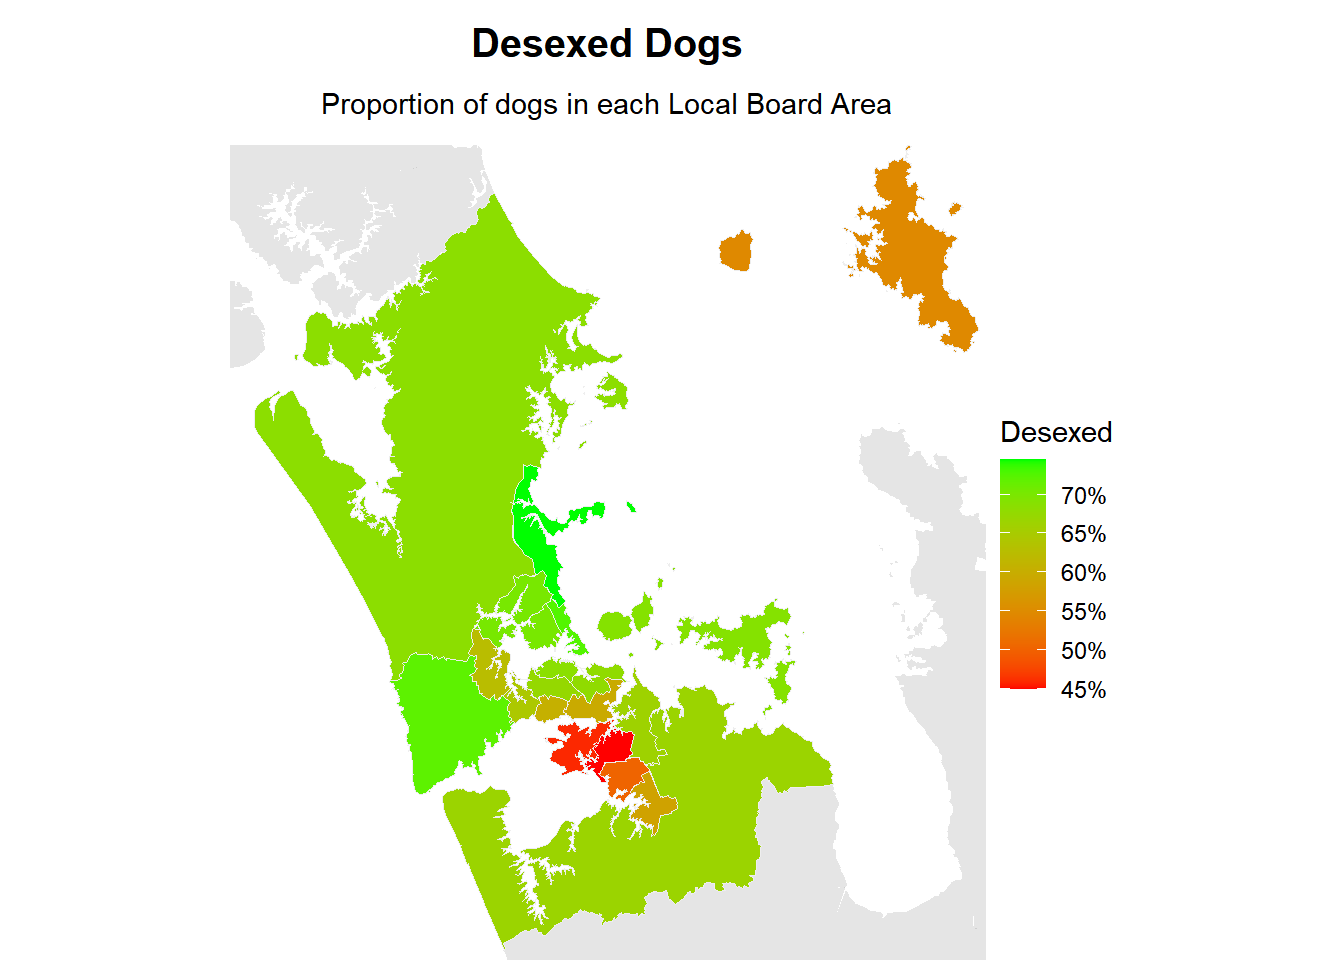
\includegraphics[keepaspectratio]{index_files/figure-latex/notebooks-mapping-map-desex-output-2.png}}

\textsubscript{Source:
\href{https://tesaunders.github.io/dog-control/notebooks/mapping-preview.html\#cell-map-desex}{Mapping}}

\pandocbounded{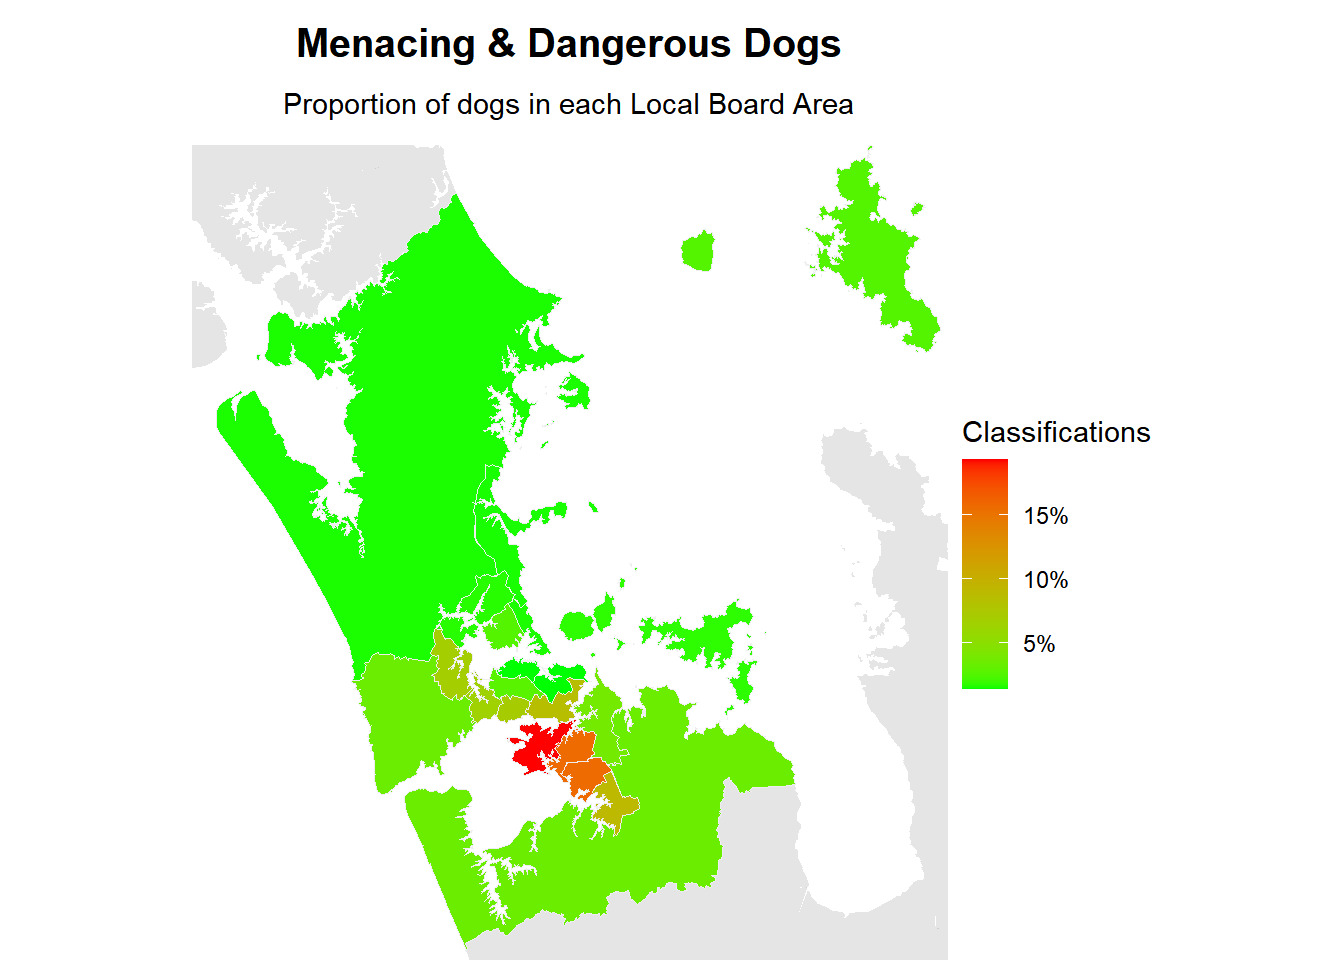
\includegraphics[keepaspectratio]{index_files/figure-latex/notebooks-mapping-map-class-output-1.png}}

\textsubscript{Source:
\href{https://tesaunders.github.io/dog-control/notebooks/mapping-preview.html\#cell-map-class}{Mapping}}

A Chi-squared test revealed which dog breeds were over represented in
each region, providing a snapshot of each region's unique breed profile.

\pandocbounded{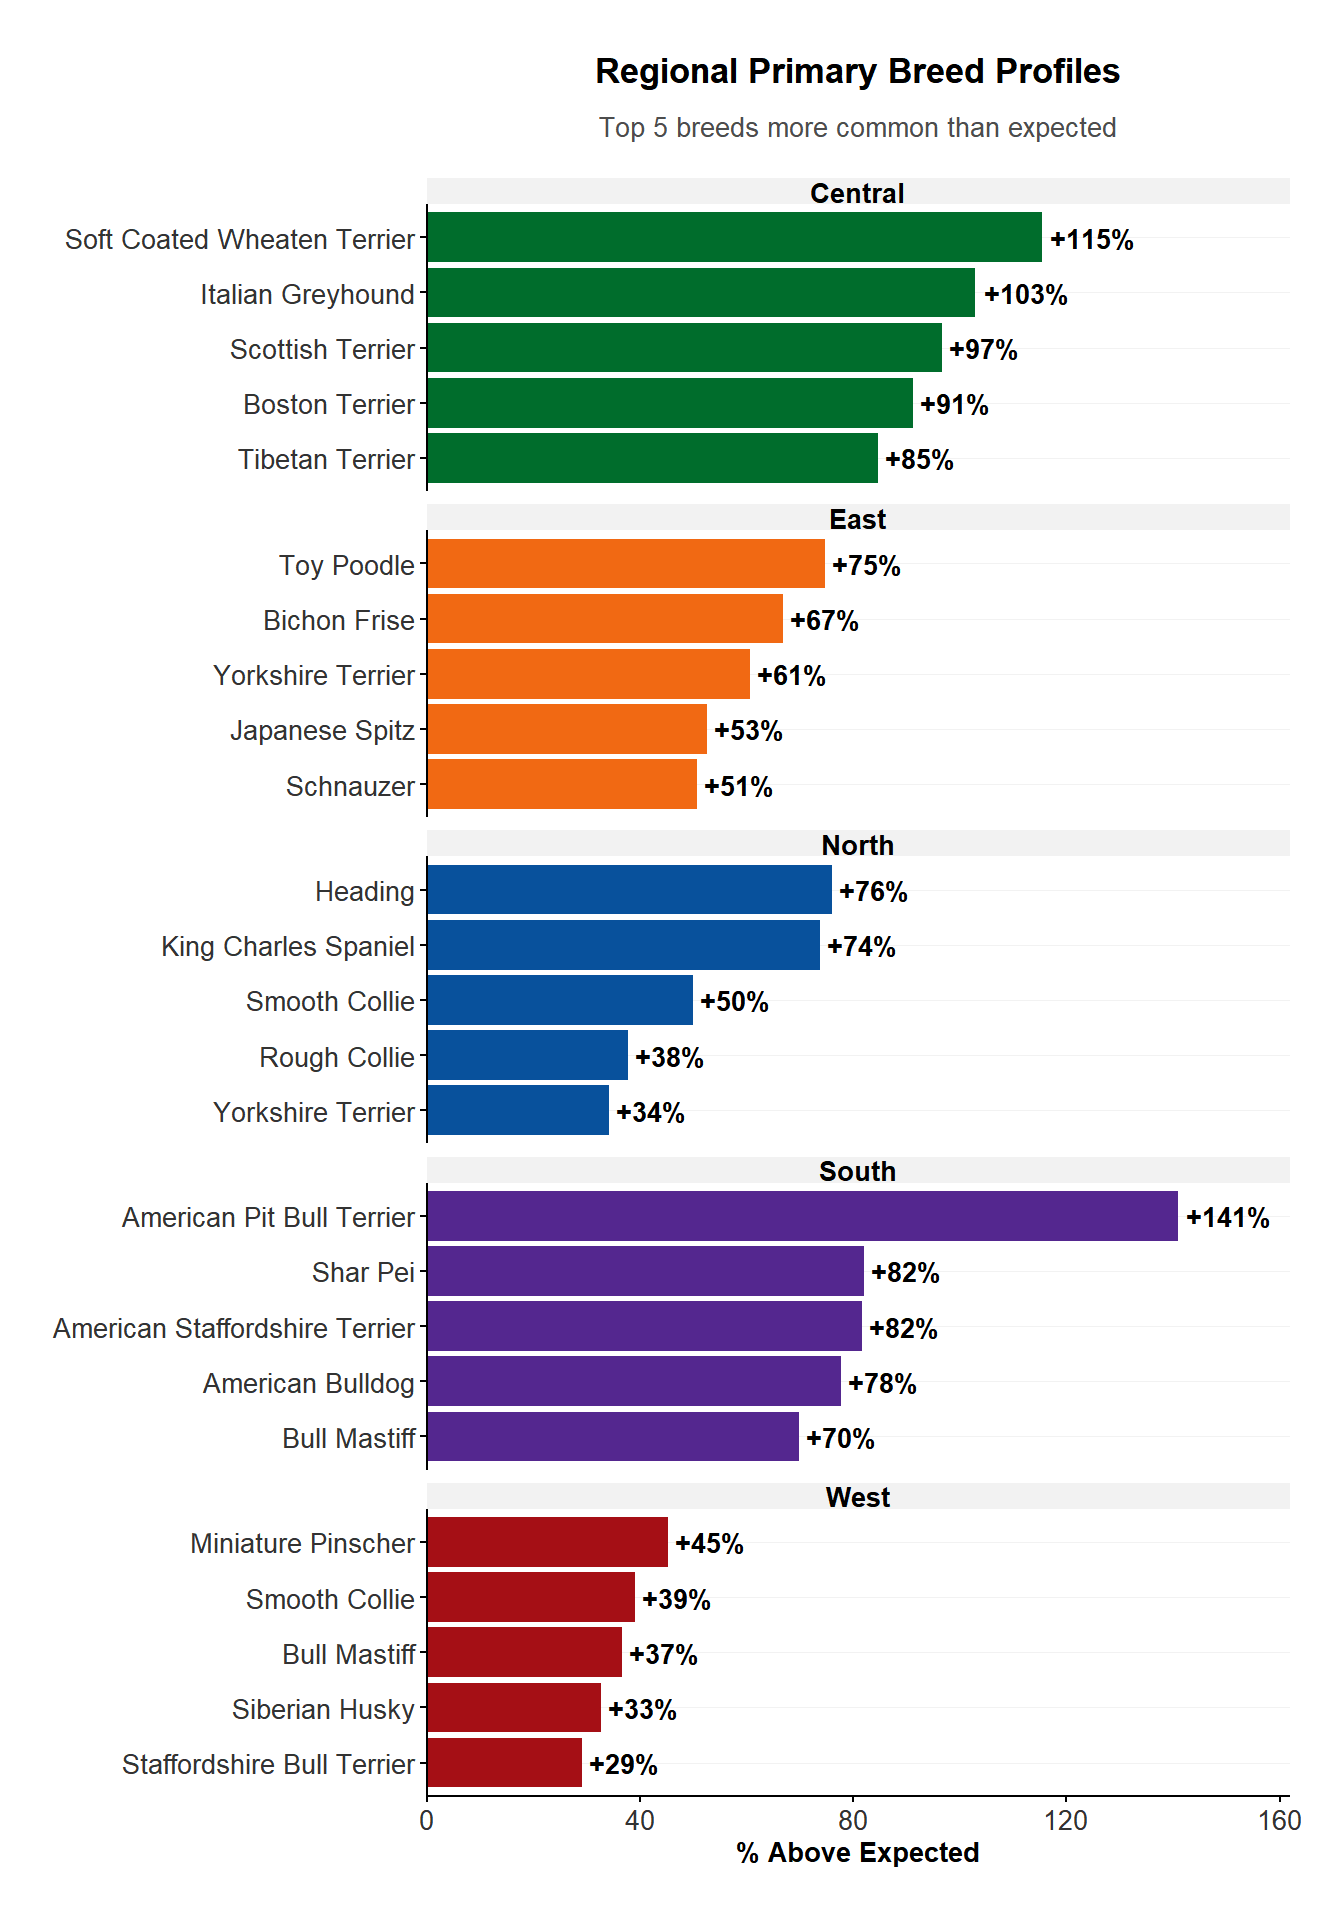
\includegraphics[keepaspectratio]{index_files/figure-latex/notebooks-data-analysis-region-breeds-output-1.png}}

\textsubscript{Source:
\href{https://tesaunders.github.io/dog-control/notebooks/data-analysis-preview.html\#cell-region-breeds}{Data
Analysis}}

Local Boards differed greatly in the rate of dog attacks, impounds, and
euthanasia of impounded dogs.

\pandocbounded{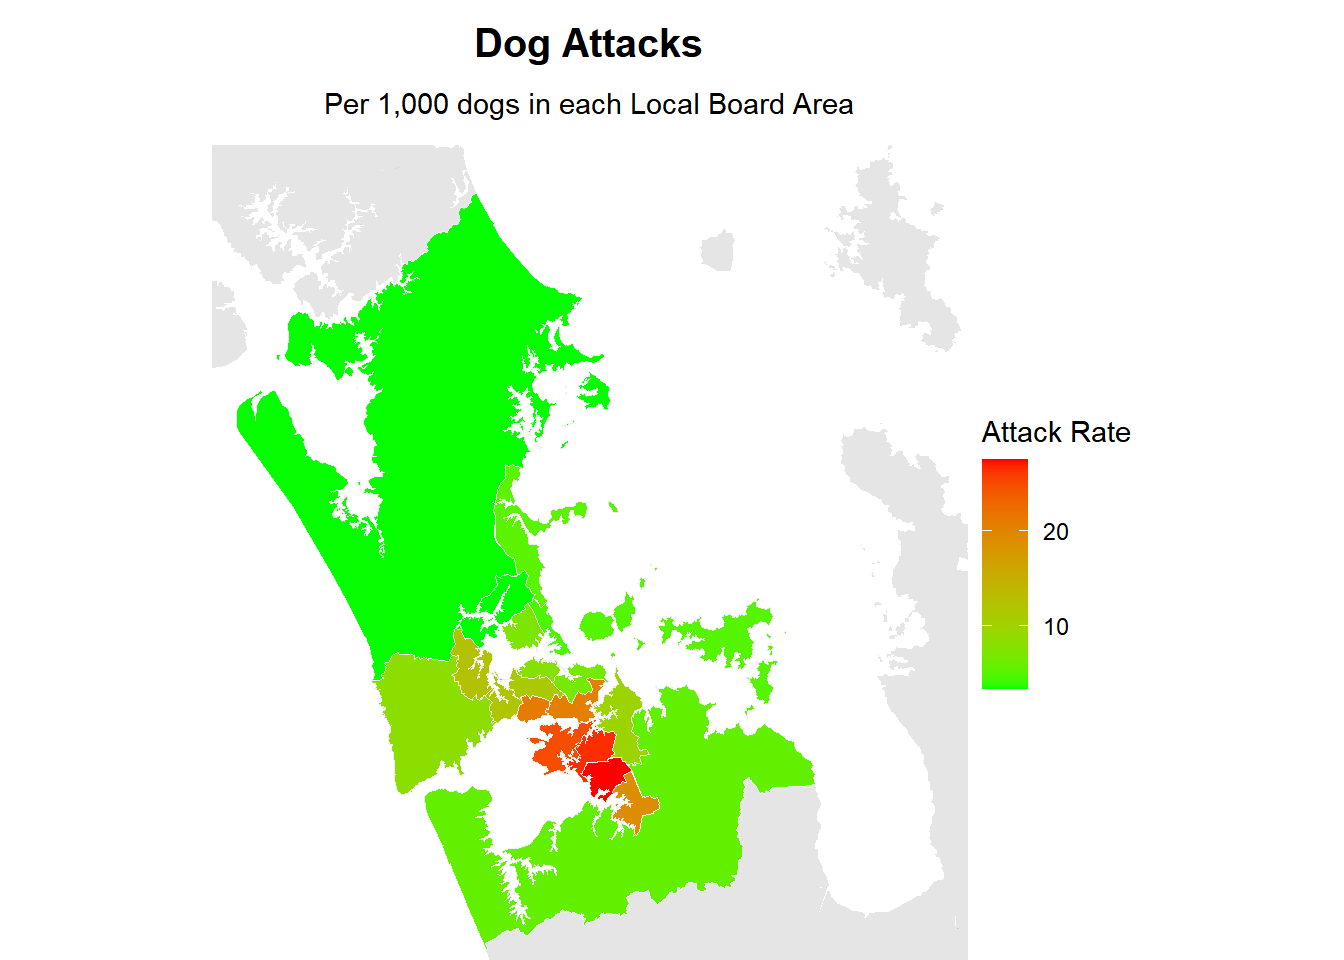
\includegraphics[keepaspectratio]{index_files/figure-latex/notebooks-mapping-map-attacks-output-1.png}}

\textsubscript{Source:
\href{https://tesaunders.github.io/dog-control/notebooks/mapping-preview.html\#cell-map-attacks}{Mapping}}

\pandocbounded{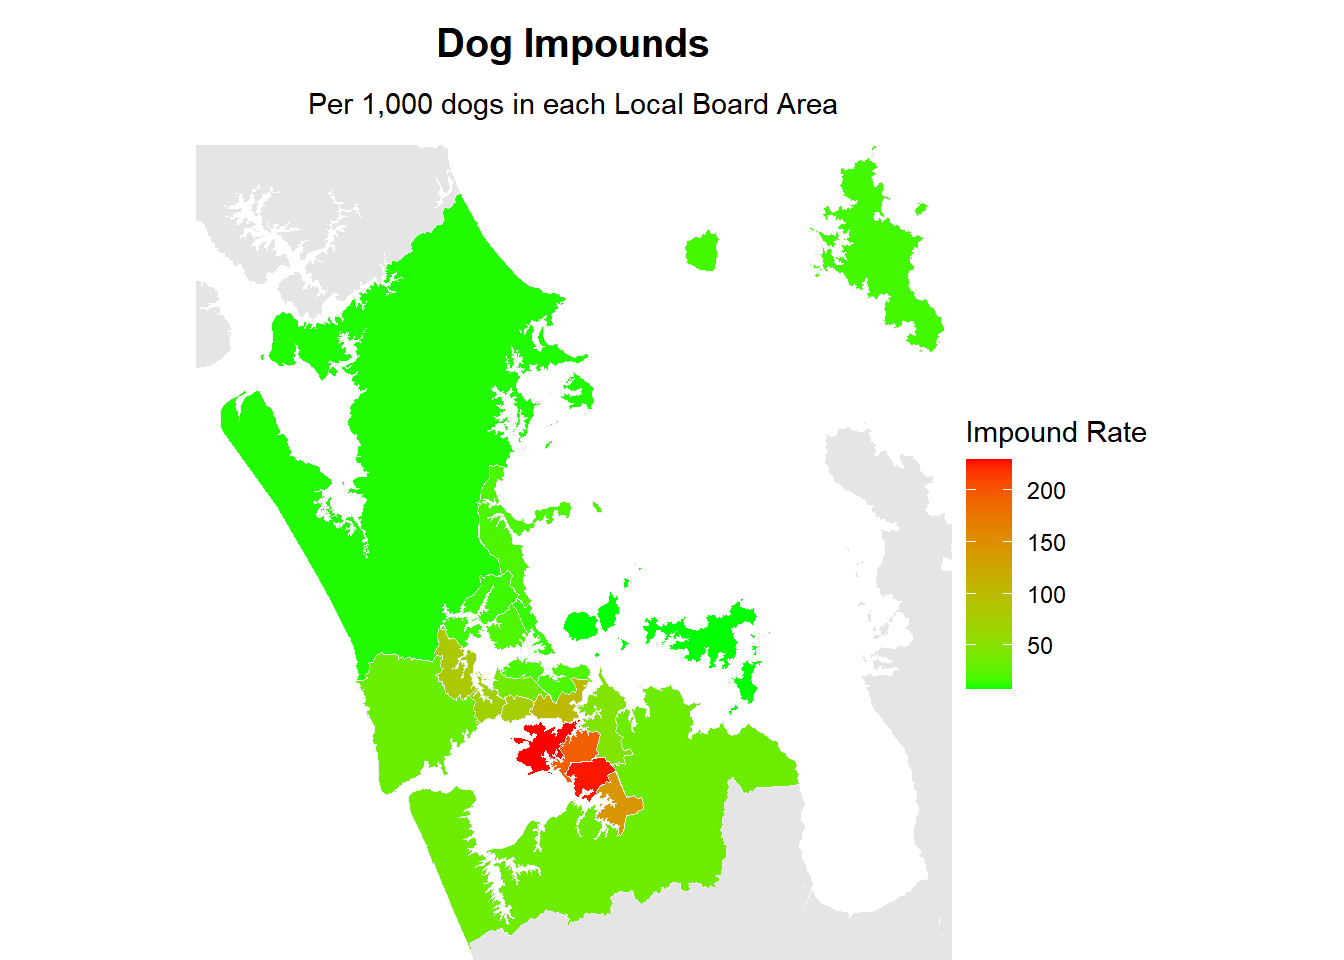
\includegraphics[keepaspectratio]{index_files/figure-latex/notebooks-mapping-map-impounds-output-1.png}}

\textsubscript{Source:
\href{https://tesaunders.github.io/dog-control/notebooks/mapping-preview.html\#cell-map-impounds}{Mapping}}

\pandocbounded{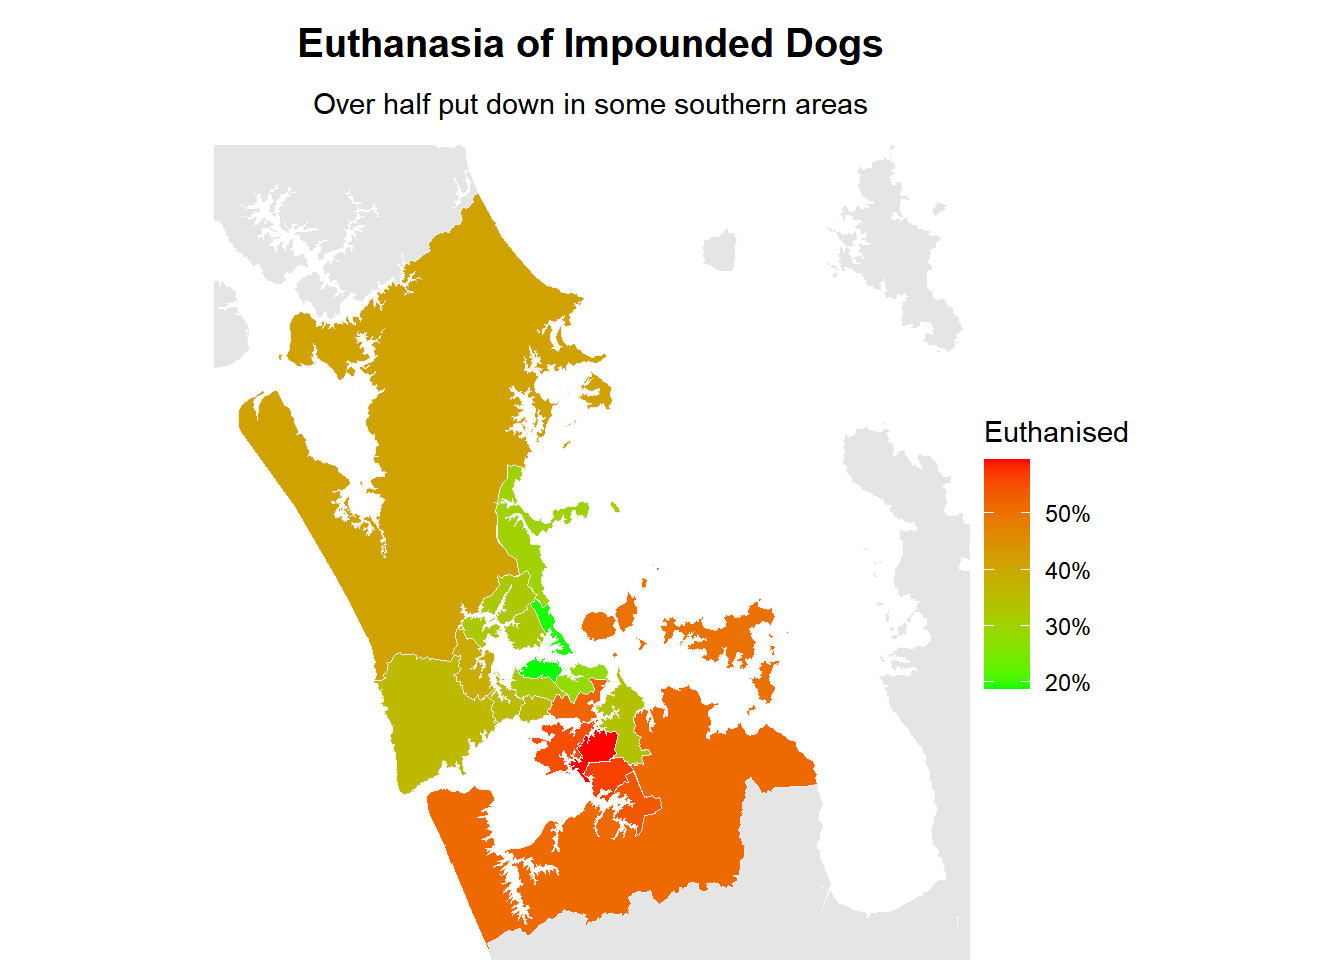
\includegraphics[keepaspectratio]{index_files/figure-latex/notebooks-mapping-map-euth-output-1.png}}

\textsubscript{Source:
\href{https://tesaunders.github.io/dog-control/notebooks/mapping-preview.html\#cell-map-euth}{Mapping}}

\pandocbounded{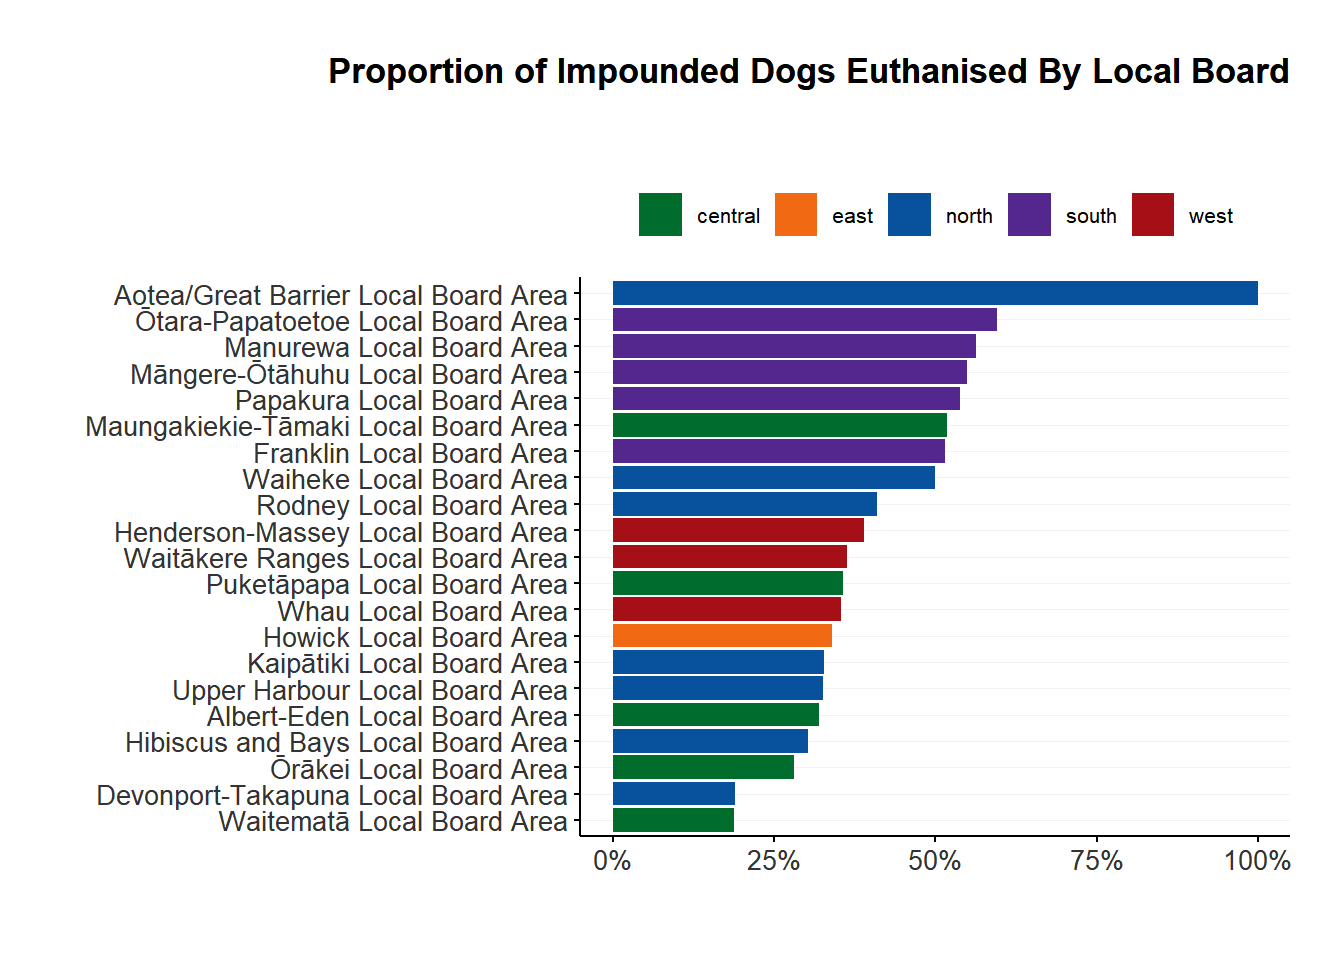
\includegraphics[keepaspectratio]{index_files/figure-latex/notebooks-data-analysis-euth-board-output-2.png}}

\textsubscript{Source:
\href{https://tesaunders.github.io/dog-control/notebooks/data-analysis-preview.html\#cell-euth-board}{Data
Analysis}}

\section{References}\label{references}

\protect\phantomsection\label{refs}
\begin{CSLReferences}{0}{1}
\bibitem[\citeproctext]{ref-anonymous2025}
\CSLLeftMargin{1. }%
\CSLRightInline{Anonymous. Far north man abel wira found guilty of
manslaughter after dogs maul neville thomson to death. \emph{RNZ}.
Published online August 26, 2025.
\url{https://www.rnz.co.nz/news/national/571133/far-north-man-abel-wira-found-guilty-of-manslaughter-after-dogs-maul-neville-thomson-to-death}}

\bibitem[\citeproctext]{ref-anonymous2023}
\CSLLeftMargin{2. }%
\CSLRightInline{Anonymous. Well-known and loved northland woman to be
farewelled after fatal dog attack. \emph{RNZ}. Published online October
16, 2023.
\url{https://www.rnz.co.nz/news/national/500293/well-known-and-loved-northland-woman-to-be-farewelled-after-fatal-dog-attack}}

\bibitem[\citeproctext]{ref-womanch2026}
\CSLLeftMargin{3. }%
\CSLRightInline{Anonymous. Woman charged after dog kills 4-year-old.
\emph{RNZ}. Published online March 9, 2026.
\url{https://www.rnz.co.nz/news/national/589066/woman-charged-after-dog-kills-4-year-old}}

\bibitem[\citeproctext]{ref-anonymous2026}
\CSLLeftMargin{4. }%
\CSLRightInline{Anonymous. Woman killed by dogs in kaihu named as
mihiata te rore. Published online February 18, 2026.
\url{https://www.rnz.co.nz/news/national/587195/woman-killed-by-dogs-in-kaihu-named-as-mihiata-te-rore}}

\bibitem[\citeproctext]{ref-anonymous2022}
\CSLLeftMargin{5. }%
\CSLRightInline{Anonymous. Killer dogs driving northland farmers from
owning sheep. \emph{RNZ}. Published online September 19, 2022.
\url{https://www.rnz.co.nz/news/country/475078/killer-dogs-driving-northland-farmers-from-owning-sheep}}

\bibitem[\citeproctext]{ref-walton2024}
\CSLLeftMargin{6. }%
\CSLRightInline{{Walton F, reporter}. Roaming dogs kill up to 30 cats in
one suburb as residents live in fear. \emph{RNZ}. Published online April
9, 2024.
\url{https://www.rnz.co.nz/news/national/513774/roaming-dogs-kill-up-to-30-cats-in-one-suburb-as-residents-live-in-fear}}

\bibitem[\citeproctext]{ref-anonymous2025a}
\CSLLeftMargin{7. }%
\CSLRightInline{Anonymous. Attacks on guide dogs leave animals too
anxious to work. \emph{RNZ}. Published online December 16, 2025.
\url{https://www.rnz.co.nz/news/national/581994/attacks-on-guide-dogs-leave-animals-too-anxious-to-work}}

\bibitem[\citeproctext]{ref-afemata2025}
\CSLLeftMargin{8. }%
\CSLRightInline{Afemata TM. 'I{'}m so scared': Crack down on roaming
dogs as residents live in fear. \emph{Pacific Media Network}. Published
online February 26, 2025.
\url{https://pmn.co.nz/read/news/i-m-so-scared-crack-down-on-roaming-dogs-as-residents-live-in-fear}}

\bibitem[\citeproctext]{ref-paddygower2025}
\CSLLeftMargin{9. }%
\CSLRightInline{Paddy Gower. {`}Causing truancy{'}: Children too afraid
to walk to school because of dangerous dogs \textbar{} stuff.
\emph{Stuffconz}. Published online September 10, 2025.
\url{https://www.stuff.co.nz/nz-news/360818146/causing-truancy-children-too-afraid-walk-school-because-dangerous-dogs}}

\bibitem[\citeproctext]{ref-departmentofinternalaffairs1996}
\CSLLeftMargin{10. }%
\CSLRightInline{Department of Internal Affairs. Dog control act 1996.
Published online May 2, 1996.
\url{https://www.legislation.govt.nz/act/public/1996/0013/latest/whole.html\#DLM374410}}

\bibitem[\citeproctext]{ref-aucklandcouncil2025a}
\CSLLeftMargin{11. }%
\CSLRightInline{Auckland Council. Dog management bylaw 2019. Published
online 2025.}

\bibitem[\citeproctext]{ref-aucklandcouncil2025b}
\CSLLeftMargin{12. }%
\CSLRightInline{Auckland Council. Policy on dogs 2025. Published online
2025.
\url{https://www.aucklandcouncil.govt.nz/content/dam/ac/docs/plans-projects-policies-reports-bylaws/misc/policy-on-dogs-2025.pdf}}

\bibitem[\citeproctext]{ref-departmentofinternalaffairs1987}
\CSLLeftMargin{13. }%
\CSLRightInline{Department of Internal Affairs. Local government
official information and meetings act 1987. Published online 1987.
\url{https://www.legislation.govt.nz}}

\bibitem[\citeproctext]{ref-saunders2026}
\CSLLeftMargin{14. }%
\CSLRightInline{Saunders TE. Akldogs: Dog control data from auckland
council. Published online March 12, 2026.
\url{https://tesaunders.github.io/akldogs/}}

\end{CSLReferences}




\end{document}
